\documentclass[
11pt, % The default document font size, options: 10pt, 11pt, 12pt
codirector, % Uncomment to add a codirector to the title page
]{charter} 

% El títulos de la memoria, se usa en la carátula y se puede usar el cualquier lugar del documento con el comando \ttitle
\titulo{Título del proyecto} 

% Nombre del posgrado, se usa en la carátula y se puede usar el cualquier lugar del documento con el comando \degreename
\posgrado{Carrera de Especialización en Sistemas Embebidos} 
%\posgrado{Carrera de Especialización en Internet de las Cosas} 
%\posgrado{Carrera de Especialización en Intelegencia Artificial}
%\posgrado{Maestría en Sistemas Embebidos} 
%\posgrado{Maestría en Internet de las cosas}

% Tu nombre, se puede usar el cualquier lugar del documento con el comando \authorname
\autor{SISE-RS versión D} 

% El nombre del director y co-director, se puede usar el cualquier lugar del documento con el comando \supname y \cosupname y \pertesupname y \pertecosupname
\director{Nombre del Director}
\pertenenciaDirector{pertenencia} 
% FIXME:NO IMPLEMENTADO EL CODIRECTOR ni su pertenencia
\codirector{John Doe} % para que aparezca en la portada se debe descomentar la opción codirector en el documentclass
\pertenenciaCoDirector{FIUBA}

% Nombre del cliente, quien va a aprobar los resultados del proyecto, se puede usar con el comando \clientename y \empclientename
\cliente{Nombre del cliente}
\empresaCliente{Empresa del cliente}

% Nombre y pertenencia de los jurados, se pueden usar el cualquier lugar del documento con el comando \jurunoname, \jurdosname y \jurtresname y \perteunoname, \pertedosname y \pertetresname.
\juradoUno{Nombre y Apellido (1)}
\pertenenciaJurUno{pertenencia (1)} 
\juradoDos{Nombre y Apellido (2)}
\pertenenciaJurDos{pertenencia (2)}
\juradoTres{Nombre y Apellido (3)}
\pertenenciaJurTres{pertenencia (3)}
 
\fechaINICIO{30 de abril de 2021}		%Fecha de inicio de la cursada de GdP \fechaInicioName
\fechaFINALPlan{18 de junio de 2021} 	%Fecha de final de cursada de GdP
\fechaFINALTrabajo{15 de mayo de 2022}	%Fecha de defensa pública del trabajo final

\def\codigo{SISE-RS}
\newcommand{\req}[1]{\textbf{[\codigo-#1]:}}

\begin{document}

\maketitle
\thispagestyle{empty}
\pagebreak


\thispagestyle{empty}
{\setlength{\parskip}{0pt}
\tableofcontents{}
}
\pagebreak


\section*{Registros de cambios}
\label{sec:registro}

\begin{table}[ht]
\label{tab:registro}
\centering
\begin{tabularx}{\linewidth}{@{}|c|X|c|@{}}
\hline
\rowcolor[HTML]{C0C0C0} 
Revisión & \multicolumn{1}{c|}{\cellcolor[HTML]{C0C0C0}Detalles de los cambios realizados} & Fecha      \\ \hline
A & Creación del documento & 27/06/2021 \\ \hline
B & Se agrega encabezado en la plantilla del documento. \newline
	Modificación de la tabla de registro de cambios. \newline
	Nuevo formato de enumeración de requisitos.\newline
	Se amplia la sección \ref{sub:perspectiva}. & 03/07/2021 \\ \hline
C & Se agregan casos de usos en el anexo & 06/07/2021 \\ \hline
D & Se conforma con las políticas de confidencialidad de INVAP. \newline
    Se modifica el título del proyecto. \newline
    Se revisan todos los requerimientos para que sean más específicos. \newline
    Se modifican los casos de uso según los nuevos requerimientos. & 11/07/2021 \\ \hline
E & Correcciones generales para la publicación de la cátedra. & 13/08/2021 \\ \hline
\end{tabularx}
\end{table}

\pagebreak

\section{1. Introducción}
\label{sec:introduccion}

\subsection{Propósito}
\label{sub:proposito}

Este documento representa una especificación de requerimientos de software para un \emph{Evaluador de microcontroladores para misiones espaciales}.
El documento está dirigido a las personas que trabajen en la esfera de: análisis, diseño, implementación o pruebas.

\subsection{Ámbito del sistema}
\label{sub:ambito}

El nombre del sistema será SISE y permitirá evaluar si el microcontrolador deseado puede tener un uso espacial.
Además, facilitará la valoración de las técnicas de mitigación de errores.
El proyecto incluirá dos módulos que funcionarán en ámbitos distintos.
Ellos serán:

\begin{itemize}
	\item Inyector por consola de comando (CCI).
	\item Proceso de dispositivo bajo prueba (DUT).
\end{itemize}

El ámbito de CCI será el ordenador del usuario; mientras que el proceso de DUT funcionará en el microcontrolador.

\subsection{Definiciones, acrónimos y abreviaturas}
\label{sub:definiciones}

\begin{enumerate}
	\item Definiciones:
		\begin{itemize}
			\item Single event effect: efecto de una partícula enérgicamente cargada sobre un microcontrolador.
			\item Single event funtional interrupt: interrupción causada por el impacto de una sola partícula que conduce a una no funcionalidad temporal.
			\item Single event upset: pulso transitorio en la lógica o circuitos de apoyo. Son \emph{soft-errors} no destructivos.
			\item Soft-error: tipo de error en donde una señal o dato es incorrecto.
		\end{itemize}
	\item Acrónimos:
		\begin{itemize}
			\item API: interfaz de programación de aplicaciones.
			\item DUT: dispositivo bajo prueba (microcontrolador).
			\item FOM: figura de mérito.
			\item IEEE: Instituto de Ingenieros Eléctricos y Electrónicos.
			\item OCD: on-chip debugger.
			\item SEE: single event effect.
			\item SEFI: single event functional interrupt.
			\item SEU: single event upset.
			\item TBD: a ser determinado.
			\item UART: universal asynchronous receiver-trasmitter.
		\end{itemize}
	\item Abreviaturas:
		\begin{itemize}
			\item Std: estándar.
		\end{itemize}
\end{enumerate}

\subsection{Referencias}
\label{sub:referencias}
INVAP - Propuesta de tesis: sistema de inyección de soft-errors.

\subsection{Visión general del documento}
\label{sub:vision}

Este documento se realizó según lo especificado en el estándar IEEE Std. 830-1998.

\section{2. Descripción general}
\label{seb:descripcion}

\subsection{Perspectiva del producto}
\label{sub:perspectiva}

El proyecto aquí especificado es independiente de otros sistemas y no tiene relación con otros productos.
Como se especificó en subsección \ref{sub:proposito}, se realizarán los siguientes módulos: CCI y Proceso de DUT.

El módulo CCI tendrá la función de generar SEFIs que introduzcan SEUs.
Los SEFI-SEU serán inyectados de forma electrónica; esto simulará los efectos de una partícula cargada que impacta en el DUT.
Como se explicó en la subsección \ref{sub:ambito}, el módulo residirá en el ordenador del usuario.
La interacción se realizará a través de una \emph{consola de línea de comandos}.
Finalmente, se podrá configurar el ensayo a realizar.

En la figura \ref{fig:CCIbloques} se puede observar el diagrama en bloques del módulo CCI.
La consola de usuario será la interfaz que el ingeniero utilice para usar el sistema.
El controlador de ensayos procesará los datos ingresados por el usuario, coordinará los SEFI-SEU y observará los reportes del DUT.
El servidor OCD se encargará de realizar lecturas de registros y las inyecciones de SEFI-SEU.
El OCD API será la interfaz entre el Controlador de ensayos y el Servidor OCD; utilizará un protocolo TBD.
La Interfaz serie capturará los informes del DUT.
Finalmente, la Persistencia de datos almacenará toda la información generada durante la ejecución del ensayo.

\begin{figure}[h!]
	\centering
	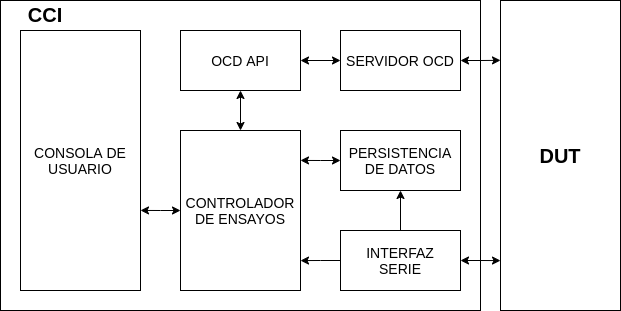
\includegraphics[width=\textwidth]{./Figuras/CCIbloques.png}
	\caption{Diagrama en bloques del módulo CCI.}
	\label{fig:CCIbloques}
\end{figure}

En la figura \ref{fig:DUTbloques} se puede observar el diagrama en bloques del módulo \emph{Proceso de DUT}.
El firmware deberá recorrer todos los periféricos del DUT.
En cada periférico se generará una operación de autovalidación.
Finalizada la verificación de todos los periféricos, el firmware enviará un reporte a través de la UART.
Finalmente, el bloque de debugger será el punto de ingreso para las SEFI-SEU.

\begin{figure}[h!]
	\centering
	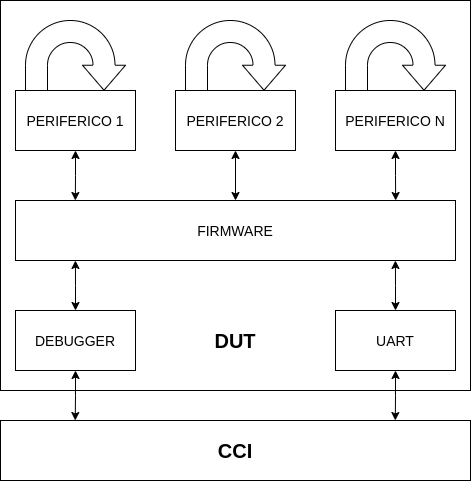
\includegraphics[width=0.7\textwidth]{./Figuras/DUTbloques.png}
	\caption{Diagrama en bloques del módulo Proceso de DUT.}
	\label{fig:DUTbloques}
\end{figure}

\subsection{Funciones del producto}
\label{sub:funcionesProducto}

El software aquí especificado brindará las siguientes funcionalidades:

\begin{enumerate}
	\item Referentes al CCI:
		\begin{enumerate}
			\item Generará de una interfaz de usuario.
			\item Permitirá configurar el ensayo a realizar.
			\item Activará el Proceso de DUT.
			\item Observará la salida del DUT.
			\item Inyectará SEFI-SEU en el DUT.
			\item Persistirá las operaciones, entradas y salidas.
			\item Generará informes del ensayo realizado.
		\end{enumerate}
	\item Referentes al Proceso de DUT:
		\begin{enumerate}
			\item Verificará el estado de los periféricos del DUT.
			\item Detectará si el DUT perdió su secuencia.
			\item Generará reportes de estado de periféricos y secuencia.
			\item Permitirá que CCI configure el alcance de la secuencia.
			\item Permitirá que CCI maneje el flujo de su secuencia.
		\end{enumerate}
\end{enumerate}

\subsection{Características de los usuarios}
\label{sub:usuarios}

Los usuarios finales de este producto son ingenieros de desarrollo de INVAP.

\subsection{Restricciones}
\label{sub:restricciones}

Las restricciones del desarrollo del sistema son las siguientes:

\begin{itemize}
	\item Utilización de repositorio con control de versiones \emph{Gitlab}.
	\item Documentación del código con \emph{Doxygen}.
	\item Utilización exclusiva del lenguaje de programación \emph{Python 3}.
\end{itemize}

\subsection{Suposiciones y dependencias}
\label{sub:suposiciones}

La suposición principal es que se tendrá acceso irrestricto al DUT seleccionado antes del día 01/01/2022.

\subsection{Requisitos futuros}
\label{sub:futuro}

N/A

\section{3. Requisitos específicos}
\label{sec:requisitos}


\subsection{Interfaces externas}
\label{sub:interfaces}

\begin{enumerate}
	\item CCI:
		\begin{enumerate}
			\item Módulo para el usuario:
				\begin{itemize}
					\item \req{001} deberá representar todos los caracteres de ISO Std. 10646.
					\item \req{002} cumplirá con las secuencias de escape especificadas en ISO Std. 6429.
					\item \req{003} usará el castellano como idioma conforme a la Real Academia Española.
					\item \req{004} se aceptarán barbarismos que conformen la interfaz con los sistemas UNIX.
					\item \req{005} no deberá producir destellos ni cambios bruscos en su intensidad lumínica.
					\item \req{006} no deberá producir sonidos
					\item Títulos:
						\begin{itemize}
							\item \req{007} los títulos deberán tener una longitud máxima de 30 caracteres.
							\item \req{008} los títulos deberán estar correctamente capitalizados.
							\item \req{009} los títulos deberán ser únicos.
						\end{itemize}
					\item Comandos:
						\begin{itemize}
							\item \req{010} el sistema se iniciará con el comando \texttt{sise.py}.
							\item \req{011} el sistema imprimirá en pantalla un manual de ayuda con el comando \texttt{sise --help}.
							\item \req{012} se podrá exportar la configuración del último ensayo realizado con el comando \texttt{sise --export=Ruta}.
							\item \req{013} se podrá importar la configuración de un ensayo a realizar con el comando \texttt{sise --import=Ruta/Archivo}.
						\end{itemize}
					\item Menú:
						\begin{itemize}
							\item \req{014} el sistema de menú tendrá una arquitectura de árbol.
							\item \req{015} la navegación entre los nodos del menú será consistente en todo el árbol.
							\item \req{016} se indicará en todo momento el nodo actual y todos los nodos que lleven a la raíz del árbol.
						\end{itemize}
				\end{itemize}
			\item Con DUT:
				\begin{itemize}
					\item \req{017} la comunicación con UART será en 9600 baudios, 8 bits de datos, 1 bit de parada y 0 bits de paridad.
					\item \req{018} la comunicación con el debugger conformará con la configuración recomendada por el fabricante.
				\end{itemize}
		\end{enumerate}
	\item Proceso de DUT:
		\begin{itemize}
			\item \req{019} la comunicación con el debugger estará disponible durante todo el flujo de la secuencia.
			\item \req{020} durante el flujo de la secuencia, la UART solo podrá transmitir información.
			\item \req{021} en el periodo entre secuencias, la UART podrá recibir y transmitir información.
		\end{itemize}
\end{enumerate}

\subsection{Funciones}
\label{sub:funciones}

\begin{enumerate}
	\item CCI:
		\begin{itemize}
			\item \req{022} detendrá la secuencia de duración $ T $ del DUT en un momento $ t $ definido como $ t \, \epsilon \, \rm I\!R^+ \wedge t \, < T$.
			\item \req{023} con la secuencia del DUT detenida, inyectará un SEFI-SEU que invertirá el valor de un bit de un registro interno.
			\item \req{024} La descripción del ensayo definirá el momento $ t $ de inyección de SEFI-SEU durante la secuencia de duración $ T $ y será un múltiplo de $\Delta t$ definido como $ \Delta t=T/N \, \forall \, N \epsilon \, \rm I\!N $.
			\item \req{025} La descripción del ensayo definirá la cantidad $ M $ de registros involucrados en la prueba.
			\item \req{026} La cantidad de secuencias $ L $ a ejecutar quedará definida como \\$ L = N \times M $.
			\item \req{027} Se ejecutará una secuencia de control sin inyección de SEFI-SEU antes de correr las $ L $ secuencias.
			\item \req{028} Por cada ejecución de una secuencia se obtendrá un valor de salida $ S $ del DUT.
			\item \req{030} Cada valor de salida $ S $ será persistido para su análisis.
			\item \req{031} Cada valor de salida $ S $ quedará asociado a su correspondiente secuencia con su inyección de SEFI-SEU y momento $ t $.
			\item \req{032} Se generará un archivo de resultados llamado\\ \texttt{resultados-AAAAMMDDHHmm.res}, siendo AAAA el año del ensayo, MM el mes, DD el día, HH la hora y mm los minutos.
			\item \req{033} El archivo de resultados acumulará los SEFI y SEU de cada registro del DUT.
			\item \req{034} El archivo de resultados acumulará los SEU de cada periférico del DUT.
			\item \req{035} El archivo de resultados indicará el FOM del registro definido como:
			$ FOM_{REG} = (1 - \frac{SEU}{SEFI}) $
			\item \req{036} El archivo de resultados indicará el FOM del DUT definido como:
			$ FOM_{DUT} = \frac{1}{M} \times \sum_{i = 1}^{i = M}FOM_{i} $ siendo $ i $ el número que representa un registro del DUT.
			\item \req{037} Se generará un archivo de histogramas llamado \\ \texttt{histogramas-AAAAMMDDHHmm.his} siendo AAAA el año del ensayo, MM el mes, DD el día, HH la hora y mm los minutos.
			\item \req{038} El archivo de histogramas tendrá una tabla que indique la frecuencia de fallos como función de los SEFIs por registro del DUT.
			\item \req{039} El archivo de histogramas tendrá una tabla que indique la frecuencia de fallos como función de los SEFIs por periférico del DUT.
		\end{itemize}
	\item Proceso de DUT:
		\begin{itemize}
			\item \req{040} deberá correr una secuencia de autoevaluación cuya ejecución durará un tiempo $ T $.
			\item \req{041} deberá producir una salida $ S $ que podrá ser un estado o una secuencia de estados.
			\item \req{042} este proceso podrá tener una entrada $ E $.
			\item \req{043} deberá evaluar el estado de los periféricos del DUT.
			\item \req{044} tendrá una función de evaluación para cada uno de los periféricos del DUT.
			\item \req{045} se podrá definir por la entrada $ E $ si se desea excluir uno o más periféricos en la secuencia.
			\item \req{046} manejará una interrupción del flujo normal de la secuencia y generará una salida $ S $ indicando la excepción, por ejemplo: interrupción por \emph{watchdog}.
			\item \req{047} la salida $ S $ utilizará la UART del DUT para ser transmitida.
			\item \req{048} la entrada $ E $ utilizará la UART del DUT para ser recibida.
		\end{itemize}
\end{enumerate}

\subsection{Requisitos de rendimiento}
\label{sub:rendimiento}

\begin{itemize}
	\item \req{049} la inyección de SEFI-SEU podrá tener un desvío en su momento $ t $ de 10 ms.
	\item \req{050} el desvío tolerado de $ t $ deberá representar como máximo el 1\% de la duración $ T $ de la secuencia del DUT.
	\item \req{051} aceptará un $ \Delta t $ que como mínimo represente el 5\% de la duración $ T $ de la secuencia del DUT.
\end{itemize}

\subsection{Restricciones de diseño}
\label{sub:restriccionesDiseño}

\begin{itemize}
	\item \req{052} se utilizará como dispositivo principal el microcontrolador seleccionado por INVAP.
	\item \req{053} se utilizará un sistema operativo de tiempo real para diseñar el Proceso de DUT.
\end{itemize}

\subsection{Atributos del sistema}
\label{sub:atributos}

\begin{enumerate}
	\item Mantenibilidad:
	\begin{itemize}
		\item \req{053} el Proceso de DUT se desarrollará con un modelo de capas.
	\end{itemize}
\end{enumerate}

\subsection{Otros requisitos}
\label{sub:otros}

N/A.

\section{4. Apéndices}
\label{sec:apendices}

%\subsection{Formatos de entrada/salida}¸

%\subsection{Resultados de análisis de costes}

\subsection{Restricciones acerca del lenguaje de programación}

El lenguaje de programación será \emph{Python 3} y el código deberá ser documentado según las recomendaciones del manual de usuario de \emph{Doxygen}.

\subsection{Casos de uso}

\begin{table}[h!]
	\label{tab:uso1}
	\caption{Caso de uso número 1}
	\begin{tabularx}{\textwidth}{|ll|X|}
		\hline
		\rowcolor[HTML]{C0C0C0} 
		\multicolumn{2}{|c|}{\cellcolor[HTML]{C0C0C0}\textbf{Título}} & \multicolumn{1}{c|}{\cellcolor[HTML]{C0C0C0}\textbf{Descripción}} \\ \hline
		\multicolumn{2}{|l|}{1. Nombre}                               & Simulación de una misión espacial                                 \\ \hline
		& 1.1 Breve descripción                   & Se simulan los años de SEFI-SEU en un lapso de 24 horas                               \\ \hline
		& 1.2 Actor principal                     & Ingeniero de INVAP                                                                    \\ \hline
		& 1.3 Disparadores                        & Comando de ejecución                                                                  \\ \hline
		\multicolumn{2}{|l|}{2. Flujo de eventos} &                                                                                       \\ \hline
		& 2.1 Flujo básico                        & \begin{tabular}[c]{@{}l@{}}
			                                                       1. El software interpreta la descripción del ensayo                    \\ 
			                                                       2. El software determina la tasa de fallos del ensayo                   \\ 
			                                                       3. El software determina la probabilidad de falla de cada registro     \\
			                                                       4. El software determina la probabilidad de falla en memoria           \\
			                                                       5. El software realiza inyecciones según los parámetros calculados     \\
			                                                       6. El software persiste todas las inyecciones realizadas               \\
			                                                       7. El software entrega un informe final                                \\
			                                                       8. El software retorna un código de tarea finalizada
		                                            \end{tabular} \\ \hline
		& 2.2 Fuljo alternativo                   & \begin{tabular}[c]{@{}l@{}}
			                                                       1. El software detecta una anormalidad en el ensayo                    \\ 
			                                                       2. El software aborta el ensayo                                        \\ 
			                                                       3. El software genera un informe de fallo                              \\
			                                                       4. El software retorna un código de error
		                                            \end{tabular} \\ \hline
		\multicolumn{2}{|l|}{3. Pre-condiciones}  & \begin{tabular}[c]{@{}l@{}}
                                                                   1. Servidor OCD corriendo                                            \\ 
                                                                   2. Servidor OCD conectado al microcontrolador                        \\ 
                                                                   3. Servidor OCD con puerto disponible
													\end{tabular}\\ \hline
		\multicolumn{2}{|l|}{4. Pos-condiciones}  & Servidor OCD liberado                                                    \\ \hline
	\end{tabularx}
\end{table}

\begin{table}[h!]
	\label{tab:uso2}
	\caption{Caso de uso número 2}
	\begin{tabularx}{\textwidth}{|ll|X|}
		\hline
		\rowcolor[HTML]{C0C0C0} 
		\multicolumn{2}{|c|}{\cellcolor[HTML]{C0C0C0}\textbf{Título}} & \multicolumn{1}{c|}{\cellcolor[HTML]{C0C0C0}\textbf{Descripción}}  \\ \hline
		\multicolumn{2}{|l|}{1. Nombre}                               & Validación de hardware                                             \\ \hline
		& 1.1 Breve descripción                   & Se obtiene la figura de mérito de un microcontrolador                                  \\ \hline
		& 1.2 Actor principal                     & Ingeniero de INVAP                                                                     \\ \hline
		& 1.3 Disparadores                        & Comando de ejecución                                                                   \\ \hline
		\multicolumn{2}{|l|}{2. Flujo de eventos} &                                                                                        \\ \hline
		& 2.1 Flujo básico                        & \begin{tabular}[c]{@{}l@{}}
			                                                       1. El usuario define la configuración del ensayo                        \\ 
			                                                       2. El ensayo se ejecuta en su totalidad                                 \\ 
			                                                       3. El sistema entrega un archivo con la figura de mérito                \\
		                                            \end{tabular} \\ \hline
		& 2.2 Fuljo alternativo                   & \begin{tabular}[c]{@{}l@{}}
			                                                       1. Durante el ensayo sucede una excepción irrecuperable                 \\ 
			                                                       2. El sistema genera un aviso de la situación por pantalla            \\ 
			                                                       3. El sistema genera un archivo con toda la información \\recolectada
		                                            \end{tabular}                                                                          \\ \hline
		\multicolumn{2}{|l|}{3. Pre-condiciones}  &                                                                                        \\ \hline
		\multicolumn{2}{|l|}{4. Pos-condiciones}  &                                                                                        \\ \hline
	\end{tabularx}
\end{table}



\end{document}
